% Monsoon Twin: the 2-page brief for Track 2, "Multiverse of Monsoon". The text follows ASD-STE100.
% Build: latexmk -pdf brief.tex   (pdflatex; packages: pgfplots, tikz, booktabs, multicol, geometry)
\documentclass[10pt]{article}
\usepackage[a4paper,margin=1.35cm,top=1.2cm,bottom=1.3cm]{geometry}
\usepackage[T1]{fontenc}
\usepackage[scaled=0.95]{helvet}
\renewcommand{\familydefault}{\sfdefault}
\usepackage{microtype,multicol,booktabs,graphicx,xcolor,enumitem,titlesec}
\usepackage{tikz,pgfplots}
\pgfplotsset{compat=1.18}
\usetikzlibrary{positioning,arrows.meta,calc}

\definecolor{ink}{HTML}{1D1D1F}\definecolor{muted}{HTML}{6E6E73}\definecolor{line}{HTML}{D1D1D6}
\definecolor{twin}{HTML}{0A66D6}\definecolor{ref}{HTML}{AEAEB2}
\definecolor{lv0}{HTML}{EDEDF0}\definecolor{lv1}{HTML}{FBE7A6}\definecolor{lv2}{HTML}{F6B77A}\definecolor{lv3}{HTML}{BE192D}

\setlength{\parindent}{0pt}\setlength{\parskip}{3pt}\setlength{\columnsep}{16pt}
\titleformat{\section}{\normalsize\bfseries\color{ink}}{\thesection}{6pt}{}
\titlespacing*{\section}{0pt}{6pt}{2pt}
\setlist{nosep,leftmargin=12pt,topsep=1pt}
\pagestyle{empty}
\linespread{1.03}

\newcommand{\fig}[1]{\par\smallskip{\footnotesize\color{muted}#1}\par}

\begin{document}

%======================================================================================================== PAGE 1
{\LARGE\bfseries Monsoon Twin}\hfill{\small\color{muted}\textbf{Team Chacha} $\cdot$ Track 2 ``Multiverse of Monsoon'' $\cdot$ Yugaantar DevForge}\\[2pt]
{\small A digital twin of the daily weather of India $\cdot$ github.com/choudharyjayesh668/monsoon-twin}
\vspace{2pt}{\color{line}\hrule}\vspace{4pt}

\begin{multicols}{2}

\section{Model design}
The twin uses the last 3 days of the weather of India on the grid of $32\times36$ points. Each point is 1 degree wide
(approximately 110\,km). The twin calculates 6 fields: temperature, rain, 2 wind fields, sea-level pressure and water
vapour. It calculates 1 day at a time. Each new day goes back into the twin as an input for the next day.

\textbf{State.} The twin does not use the weather values directly. It uses the difference from the long-term average
of that calendar day (the ``anomaly''), divided by a scale for each field. The long-term average is the same as the
average of the organisers.

\textbf{Network.} A small convolutional network calculates the change of the anomaly for 1 day
(Figure~1). It has a $3\times3$ input layer, 5 residual $3\times3$ blocks and a $1\times1$ output layer: 0.77 million
weights. It has no pooling and no attention. Thus, a change moves a maximum of 6 grid points in 1 day.
A shock cannot jump across India in 1 step. A test makes sure of this limit.

\begin{center}
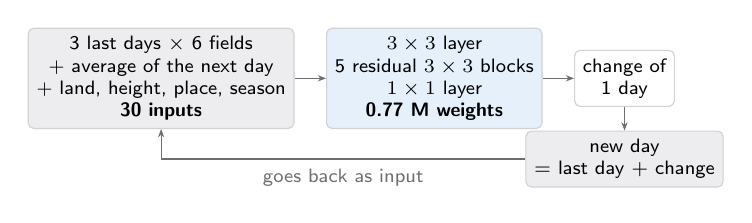
\begin{tikzpicture}[font=\scriptsize, box/.style={draw=line, rounded corners=2pt, fill=white, align=center, inner sep=3pt},
  arr/.style={-{Stealth[length=3pt]}, color=muted}]
  \node[box, fill=lv0] (in) {3 last days $\times$ 6 fields\\+ average of the next day\\+ land, height, place, season\\\textbf{30 inputs}};
  \node[box, right=4mm of in, fill=twin!10] (net) {$3\times3$ layer\\5 residual $3\times3$ blocks\\$1\times1$ layer\\\textbf{0.77 M weights}};
  \node[box, right=4mm of net] (out) {change of\\1 day};
  \node[box, below=3mm of out, fill=lv0] (new) {new day\\$=$ last day $+$ change};
  \draw[arr] (in) -- (net); \draw[arr] (net) -- (out); \draw[arr] (out) -- (new);
  \draw[arr] (new.west) -| node[pos=0.25, below, color=muted]{goes back as input} ($(in.south)+(0,0)$);
\end{tikzpicture}
\fig{Figure 1. One step of the twin. The step repeats for each day, for a maximum of 14 days.}
\end{center}

\textbf{Training.} The loss is the score of the organisers: the error is divided by the error of the better simple
forecast. First, the twin learns 1 day. Then it learns 4 days in sequence from its own output. We trained it with MLX on
an Apple GPU, in approximately 19 minutes. We developed on 2005--2017, set the limits on 2018--2019 and measured
1 time on 2020--2021. The final weights use the same procedure on 2005--2021.

\textbf{Heavy rain.} Where the forecast rain is more than a limit for that day (8.5\,mm on day 1, approximately 6.5\,mm on day 8), the output increases it to just above 10\,mm/day.
This decision is for each grid point. The twin does not use the increased rain for the next day.

\section{How the twin prevents drift and blur}
\textbf{Drift.} The anomalies stay near the long-term average, thus each day has a fixed reference. The training on
4 days in sequence teaches the twin how fast an anomaly becomes small. Rain cannot be less than 0 in the calculation.
At the output, limits remove impossible values. In all 721 test windows, all 14 days were correct: no NaN, no Inf,
no negative rain, temperature always in the limits of the organisers.

\textbf{Blur.} When a model makes the mean error small, its forecast can become flat. The grader compares the spatial variance on
day 8 with the real variance and needs 40\%. Figure~2 shows that the twin keeps most of the detail. Rain keeps
the least detail.

\begin{center}
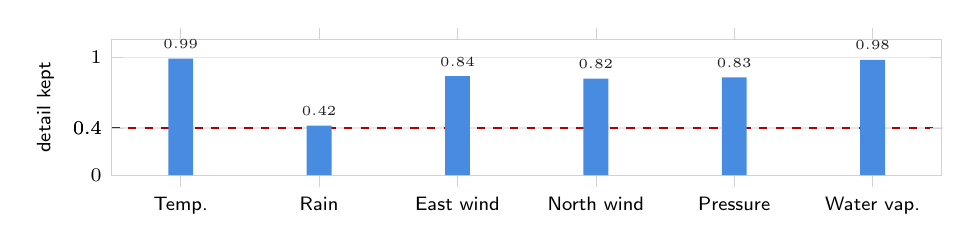
\begin{tikzpicture}
\begin{axis}[ybar, width=\linewidth, height=3.3cm, bar width=9pt, ymin=0, ymax=1.15,
  symbolic x coords={Temp.,Rain,East wind,North wind,Pressure,Water vap.}, xtick=data,
  ticklabel style={font=\scriptsize}, ylabel={\scriptsize detail kept}, ytick={0,0.4,1},
  axis line style={line}, tick style={line}, ymajorgrids, grid style={line!50},
  nodes near coords, every node near coord/.append style={font=\tiny, color=ink},
  extra y ticks={0.4}, extra y tick style={grid=major, grid style={red!70!black, dashed}}]
  \addplot[fill=twin!75, draw=none] coordinates {(Temp.,0.99) (Rain,0.42) (East wind,0.84) (North wind,0.82) (Pressure,0.83) (Water vap.,0.98)};
\end{axis}
\end{tikzpicture}
\fig{Figure 2. Spatial variance on day 8, divided by the real variance (mean of the 9 demo windows). Dashed line:
the limit of the organisers (0.40).}
\end{center}

\textbf{Skill.} The skill is $1-\mathrm{RMSE}/\mathrm{RMSE}_{\mathrm{best}}$, where ``best'' is the better of ``repeat
yesterday'' and the long-term average. Above 0, the twin is better than both (Figure~3).

\begin{center}
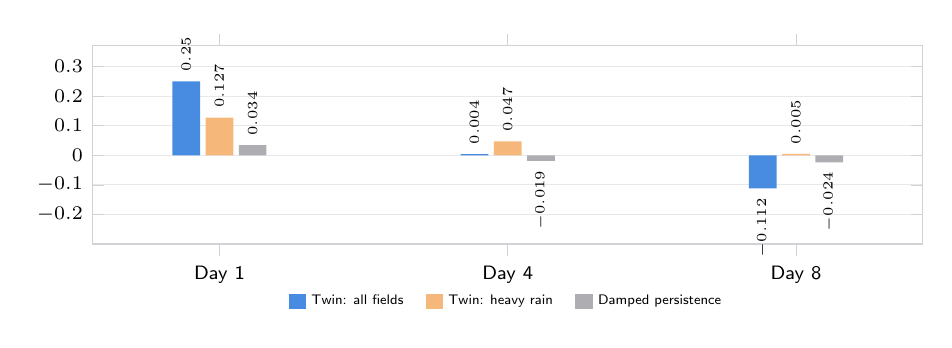
\begin{tikzpicture}
\begin{axis}[ybar, width=\linewidth, height=4.1cm, bar width=10pt, ymin=-0.3, ymax=0.37,
  symbolic x coords={Day 1,Day 4,Day 8}, xtick=data, enlarge x limits=0.22,
  ticklabel style={font=\scriptsize}, ytick={-0.2,-0.1,0,0.1,0.2,0.3}, yticklabel style={/pgf/number format/fixed},
  axis line style={line}, tick style={line}, ymajorgrids, grid style={line!50},
  legend style={font=\tiny, draw=none, at={(0.5,-0.2)}, anchor=north, legend columns=3, /tikz/every even column/.append style={column sep=6pt}},
  legend image code/.code={\fill[#1] (0cm,-0.08cm) rectangle (0.22cm,0.1cm);},
  nodes near coords, every node near coord/.append style={font=\tiny, rotate=90, anchor=west, /pgf/number format/fixed, /pgf/number format/precision=3},
  visualization depends on=y \as \yv, every node near coord/.append style={anchor={\ifdim\yv pt<0pt east\else west\fi}}]
  \addplot[fill=twin!75, draw=none] coordinates {(Day 1,0.250) (Day 4,0.004) (Day 8,-0.112)};
  \addplot[fill=lv2, draw=none] coordinates {(Day 1,0.127) (Day 4,0.047) (Day 8,0.005)};
  \addplot[fill=ref, draw=none] coordinates {(Day 1,0.034) (Day 4,-0.019) (Day 8,-0.024)};
  \legend{Twin: all fields, Twin: heavy rain, Damped persistence}
\end{axis}
\end{tikzpicture}
\fig{Figure 3. Skill on 2020--2021, which the development model did not see (721 windows). The twin is better than
``repeat yesterday'' on day 4 by 0.225: it passes the qualifying test.}
\end{center}

\section{Failure modes}
\begin{enumerate}
\item \textbf{Rain with more water vapour.} With the Bay of Bengal shock, a single heavy-rain cell can change by more
  than 5 standard deviations (38\,mm/day). This occurs in approximately 26\% of the windows.
\item \textbf{The weak-wind shock becomes too small.} It moves far enough by days 4--8 in only approximately half of
  the windows.
\item \textbf{Day 8 is near the long-term average.} After day 4, the skill comes from a correct decrease of the anomaly,
  not from new weather. On day 8, the twin is a little worse than the long-term average.
\item \textbf{Rain detail.} On day 8, rain keeps only 42\% of the real variance, near the limit of 40\%.
\item \textbf{Leap years.} The requests do not tell the year. Thus, the long-term average is 1 day late from March.
\item \textbf{The edge of the grid.} The twin cannot see weather from outside the grid. The edges become worse first.
\item \textbf{Overfitting.} On its training years, the twin gets much better scores (0.17 against 0.05).
\end{enumerate}

\end{multicols}

\newpage
%======================================================================================================== PAGE 2
{\Large\bfseries Visualisation and impact: flood risk}\hfill{\small\color{muted}Team Chacha $\cdot$ Monsoon Twin $\cdot$ page 2}
\vspace{2pt}{\color{line}\hrule}\vspace{5pt}

\begin{minipage}[t]{0.495\linewidth}
  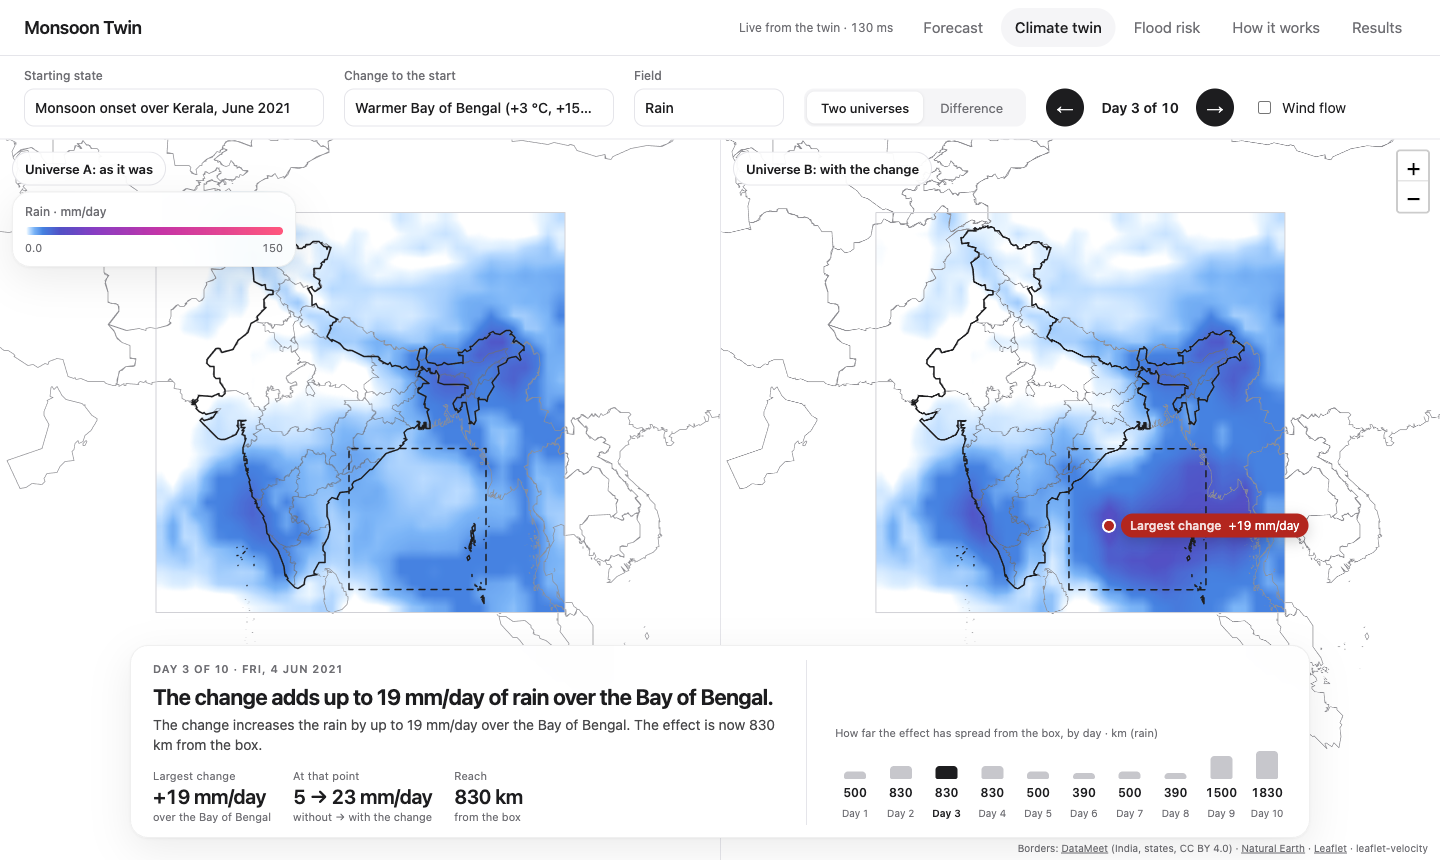
\includegraphics[width=\linewidth]{figures/twin.png}
  \fig{Figure 4. Climate twin page. Universe A (left) and universe B with a Bay of Bengal 3\,\textdegree C warmer
  (right), day 3. The panel tells the largest change (+19\,mm/day), the values at that point (5\,$\rightarrow$\,23)
  and how far the effect has moved (830\,km).}
\end{minipage}\hfill
\begin{minipage}[t]{0.495\linewidth}
  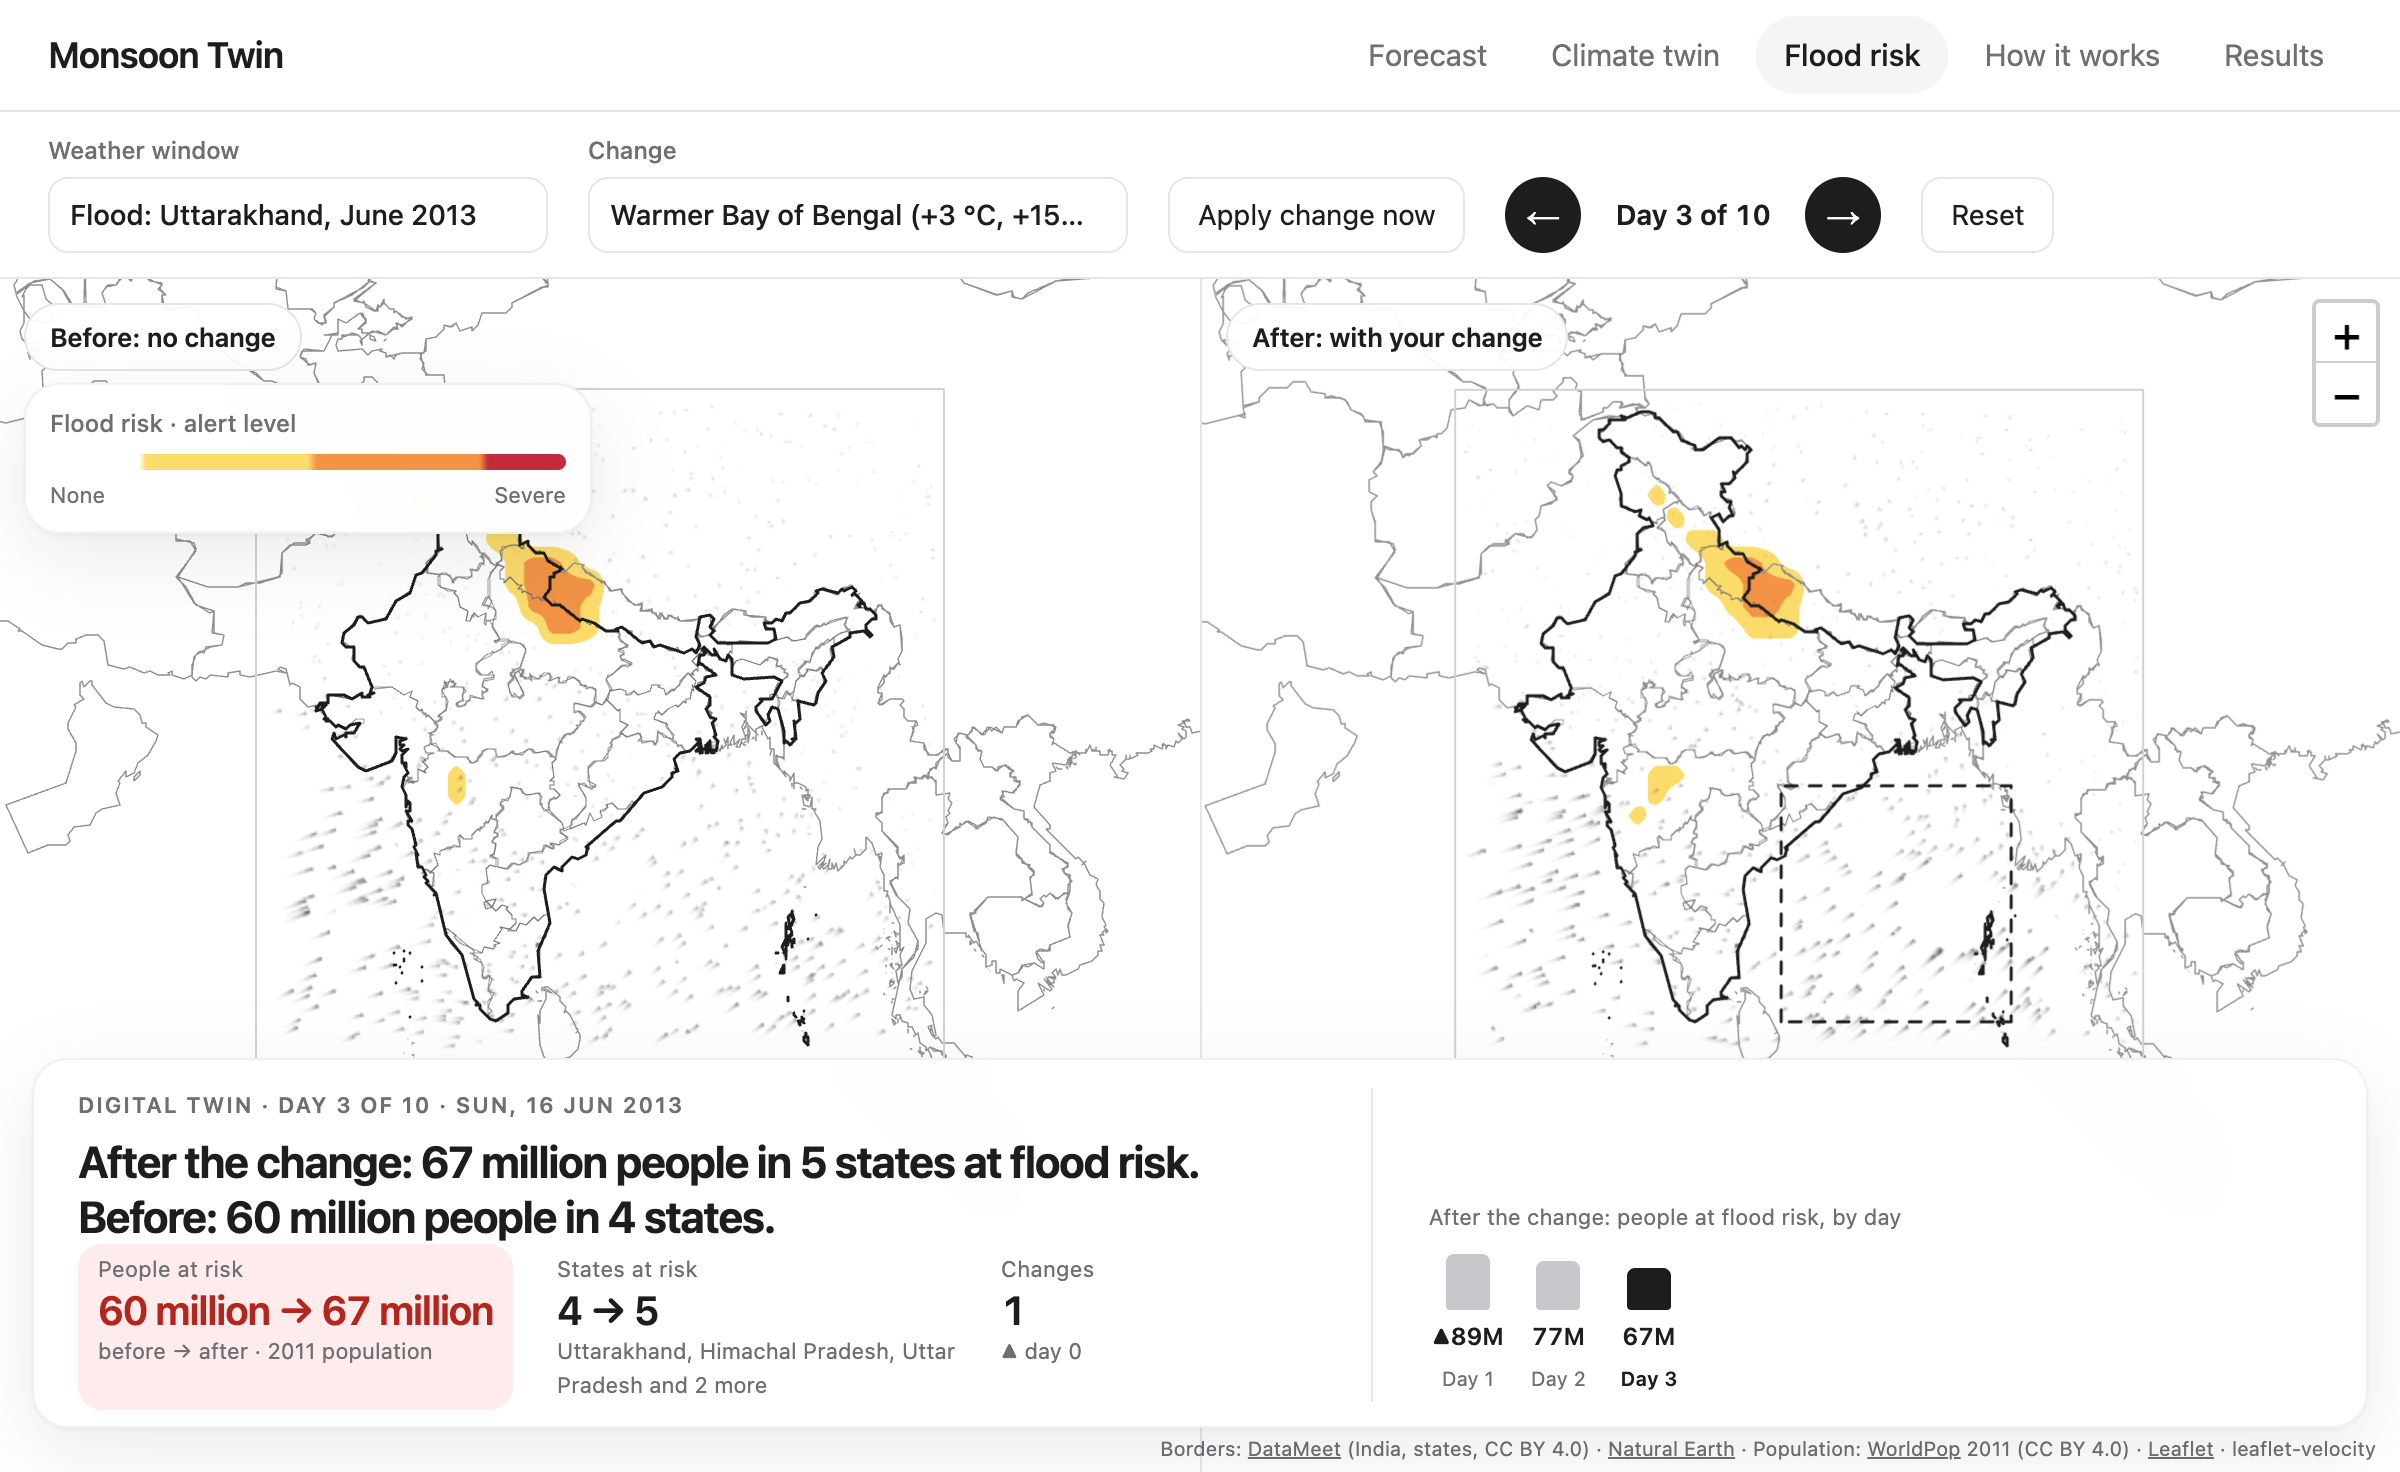
\includegraphics[width=\linewidth]{figures/flood.png}
  \fig{Figure 5. Flood risk page, Uttarakhand 2013, day 3, Bay of Bengal 3\,\textdegree C warmer: 60 to 67
  million people, and 4 to 5 states, at flood risk.}
\end{minipage}

\begin{multicols}{2}

\section{Visualisation}
The demo is a website with 3 map pages. Each map comes from the server of the twin at the time of the request.
The demo does not show saved results. It works without an internet connection.

\begin{itemize}
\item \textbf{Forecast.} The real weather and the twin forecast are side by side, with the same colours. The panel
  shows the skill of each day. The page uses the method of the organisers' kit. Its values are the same as the kit
  values in all 90 tested window-days.
\item \textbf{Climate twin} (Figure~4). The same 3 real days give 2 universes. Universe B has a change to the last day:
  a shock of the organisers, or your own change. You select a region (or click on the map), a field and an amount.
  The page shows the 2 universes or their difference. A change of 0 gives the same forecast, bit for bit.
\item \textbf{Flood risk} (Figure~5). A digital twin with 2 copies of the weather: \emph{Before} without a change
  and \emph{After} with your change. Each press of $\rightarrow$ calculates 1 more day for both, up to 10 days.
\end{itemize}
The borders of India come from DataMeet and agree with the Survey of India. The twin answers a 10-day request in
approximately 0.1\,s on a laptop CPU and uses 218\,MB of memory.

\section{Impact use case: flood risk what-if}
\textbf{User.} A state or district disaster management team. It needs to know: which states are at flood risk, how
many people live there, and how a change to the weather changes this.

\textbf{Method.} For each grid point, the module adds the rain of 3 days. It compares this value with the rain of
3 days that is rare for that place and month (2005--2021). There are 3 levels: \emph{watch} (rarer than 97\%, more than
40\,mm), \emph{warning} (99\%, 70\,mm) and \emph{severe} (99.7\%, 100\,mm). A state is at risk when an alert covers
10\% of its area. The population is WorldPop 2011 (CC BY 4.0).

\textbf{What-if.} The 2 copies start from the same 3 real days. You apply a change to \emph{After} at the start or on
any later day: a shock of the organisers, or your own region, field and amount. The twin then calculates each next day
from its own last 3 days, with 1 live request per copy. The page shows the people and the states at risk, before and
after. On Uttarakhand 2013, a Bay of Bengal 3\,\textdegree C warmer changes day 3 from 60 to 67 million people, and
from 4 to 5 states.

\textbf{Limits.} The module uses rain only: no rivers, dams or drainage. A grid point is 110\,km wide, thus the alert
is for a state, not for a town. The population is from 2011, thus the number of people today is larger. The flood
windows are in the training years of the final twin, thus the twin looks better on them than on a new flood.

\end{multicols}
\end{document}
